\documentclass{article} % For LaTeX2e
\usepackage{nips14submit_e,times}
\usepackage{amsmath}
\usepackage{amsthm}
\usepackage{amssymb}
\usepackage{mathtools}
\usepackage{hyperref}
\usepackage{url}
\usepackage{algorithm}
\usepackage[noend]{algpseudocode}
%\documentstyle[nips14submit_09,times,art10]{article} % For LaTeX 2.09

\usepackage{bbm}
\usepackage{graphicx}
\usepackage{caption}
\usepackage{subcaption}
\usepackage{MnSymbol}

\def\eQb#1\eQe{\begin{eqnarray*}#1\end{eqnarray*}}
\def\eQnb#1\eQne{\begin{eqnarray}#1\end{eqnarray}}
\providecommand{\e}[1]{\ensuremath{\times 10^{#1}}}
\providecommand{\pb}[0]{\pagebreak}
\DeclarePairedDelimiter\ceil{\lceil}{\rceil}
\DeclarePairedDelimiter\floor{\lfloor}{\rfloor}

\newcommand{\E}{\mathrm{E}}
\newcommand{\Var}{\mathrm{Var}}
\newcommand{\Cov}{\mathrm{Cov}}

\def\Qb#1\Qe{\begin{question}#1\end{question}}
\def\Sb#1\Se{\begin{solution}#1\end{solution}}

\newenvironment{claim}[1]{\par\noindent\underline{Claim:}\space#1}{}
\newtheoremstyle{quest}{\topsep}{\topsep}{}{}{\bfseries}{}{ }{\thmname{#1}\thmnote{ #3}.}
\theoremstyle{quest}
\newtheorem*{definition}{Definition}
\newtheorem*{theorem}{Theorem}
\newtheorem*{lemma}{Lemma}
\newtheorem*{question}{Question}
\newtheorem*{preposition}{Preposition}
\newtheorem*{exercise}{Exercise}
\newtheorem*{challengeproblem}{Challenge Problem}
\newtheorem*{solution}{Solution}
\newtheorem*{remark}{Remark}
\usepackage{verbatimbox}
\usepackage{listings}
\usepackage{mathrsfs}
\title{ProbLimI: \\
Problem Set III}


\author{
Youngduck Choi \\
CIMS \\
New York University\\
\texttt{yc1104@nyu.edu} \\
}


% The \author macro works with any number of authors. There are two commands
% used to separate the names and addresses of multiple authors: \And and \AND.
%
% Using \And between authors leaves it to \LaTeX{} to determine where to break
% the lines. Using \AND forces a linebreak at that point. So, if \LaTeX{}
% puts 3 of 4 authors names on the first line, and the last on the second
% line, try using \AND instead of \And before the third author name.

\newcommand{\fix}{\marginpar{FIX}}
\newcommand{\new}{\marginpar{NEW}}

\nipsfinalcopy % Uncomment for camera-ready version

\begin{document}


\maketitle

\begin{abstract}
This work contains solutions to the exercises of the problem set III. The
chosen problems are 1,3, and 4.
\end{abstract}

\bigskip

\begin{question}[1]
\hfill
\begin{figure}[h!]
  \centering
    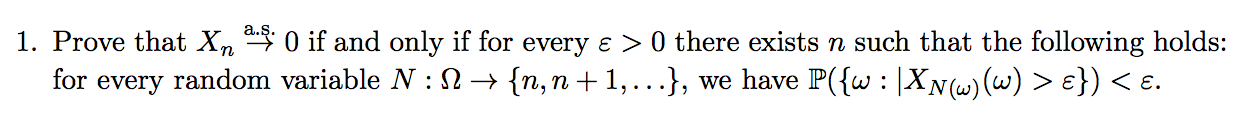
\includegraphics[width=0.7\textwidth]{prob-e3-p1.png}
\end{figure}
\end{question}
\begin{solution} \hfill \\
Fix $\epsilon > 0$.  
Choose $C \in \mathscr{F}$ such that $\mathbb{P}(C) = 0$,
and for any $w \in \Omega \setminus C$, 
there exists $n(w) \geq 1$, such that $|X_n(w)| < \epsilon$, whenever $n \geq n(w)$.
Set $n(w) = \infty$ for each $w \in C$.
Now, for each $n \geq 1$, define
\eQb
A_n := \{ w: n(w) > n\}. 
\eQe 
It follows that $\{ A_n \}$ is descending and $\bigcap_n A_n = C$. Therefore, by
continuity of probability, there exists $n_0$ such that $\mathbb{P}(A_{n_0}) < 
\epsilon$. Then, it follows that, for any $N:\Omega \to \{ n_0,...\}$, 
\eQb
\mathbb{P}(\{w: |X_{N(w)}(w)| > \epsilon\} &\leq& \mathbb{P}(A_{n_0}) < \epsilon. 
\eQe  
The first inequality holds, because, for all $w \in \Omega$ and $N:\Omega 
\to \{n_0,...\}$,
\eQb
X_{N(w)}(w) > \epsilon &\implies n_0 \leq N(w) < n(w), 
\eQe
as required. 

\bigskip

Conversely, suppose that $\{x_n\}$ does not converge almost surely to $0$. Choose
$E \in \mathscr{F}$ such that $\mathbb{P}(E) > 0$, and $0 < \epsilon < \mathbb{P}(E)$
such that for any $w \in E$, there exists $\{n_k\}$ such that
\eQb
|x_{n_k}(w)| > \epsilon , \>\> \text{ for any } \>\> k \geq 1.
\eQe  
Fix $n \geq 1$. Define $N: \Omega \to \{n,...\}$ by 
\eQb
w \mapsto \inf\{ n_k \>: \> 
n_k \geq n \>\> \text{and} \>\> |x_{n_k}(w)| > \epsilon \} 
\eQe
if $w \in E$ and $w \mapsto n$ otherwise.
Then, it follows that
\eQb
\mathbb{P}(\{w : |X_{N(w)}(w)| > \epsilon\}) &\geq& \mathbb{P}(E) > \epsilon, 
\eQe
and we are done. \hfill $\qed$


\end{solution}

\newpage

\begin{question}[2]
\hfill
\begin{figure}[h!]
  \centering
    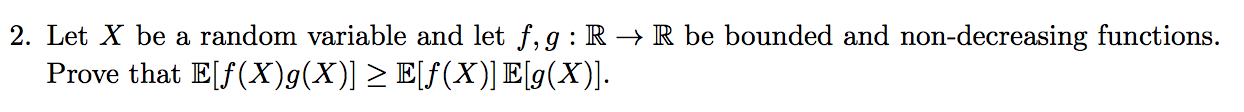
\includegraphics[width=0.7\textwidth]{prob-e3-p2.png}
\end{figure}
\end{question}
\begin{solution} \hfill \\
\end{solution}

\newpage

\begin{question}[3]
\hfill
\begin{figure}[h!]
  \centering
    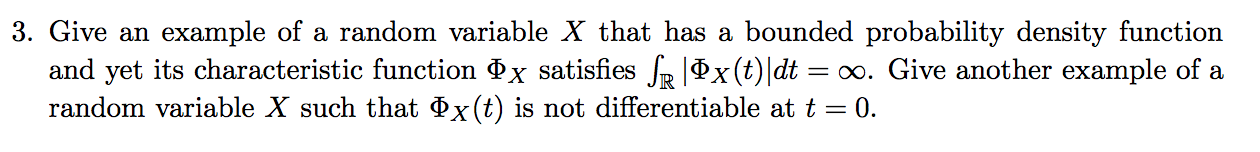
\includegraphics[width=0.7\textwidth]{prob-e3-p3.png}
\end{figure}
\end{question}
\begin{solution} \hfill \\
Exponential distribution with density $f(x) = e^{-x}$ 
has a bounded density function, but 
\eQb
\int_{\mathbb{R}} |\dfrac{1}{1-it}| dt = \int_{\mathbb{R}} \dfrac{1}{\sqrt{1+t^2}}
dt = \infty 
\eQe
Cauchy distribution with density $f(x) = \dfrac{1}{\pi} \dfrac{1}{1+x^2}$ 
has the characteristic function $\phi(t) = e^{-|t|}$, which is not differentiable 
at $0$. \hfill $\qed$
\end{solution}

\newpage

\begin{question}[4]
\hfill
\begin{figure}[h!]
  \centering
    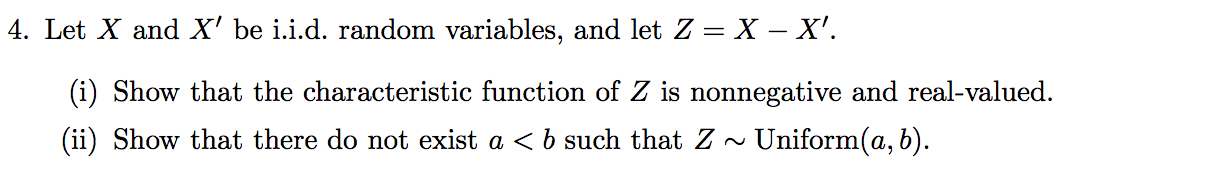
\includegraphics[width=0.7\textwidth]{prob-e3-p4.png}
\end{figure}
\end{question}
\begin{solution} \hfill \\
\textbf{(i)}
We assume basic Fourier analysis here.
Fix $t \in \mathbb{R}$.
By independence, we have 
\eQb
\phi_{Z}(t) &=& \phi_{X}(t)\phi_{X'}(-t) \>\> (*)
\eQe
Now, observe that for any random variable $Y$ and $s \in \mathbb{R}$, we have
\eQb
\phi_Y(-s) &=& \mathbb{E}\cos(sY) - i\sin(sY) = \overline{\mathbb{E}\cos(sY) + 
i\sin(sY)} = \overline{\phi_{Y}(s)} 
\eQe
As $X'$ and $X$ are identically distributed, from $(*)$, and the above, 
we obtain
\eQb
\phi_{Z}(t) = \phi_{X}(t) \overline{\phi_{X}(t)} = |\phi_{X}(t)|^2.
\eQe 
Since $t \in \mathbb{R}$ was arbitrary, we have shown $Z \geq 0$ as required.

\bigskip

\textbf{(ii)} Suppose otherwise. Then, $Z$ has a density $f = \dfrac{1}{b-a}1_{[a,b]}$.
Then, by a change of variable, for $t \neq 0$,
\eQb
\phi_{Z}(t) &=& \int_{a}^{b} \dfrac{e^{itz}}{b-a} dz = \dfrac{e^{itb}-e^{ita}}{
it(b-a)},
\eQe
and $\phi_{Z}(0) = 1$. 
From $(i)$, we deduce that, for any $t \neq 0$, 
\eQb
\cos(tb) &=& \cos(ta). 
\eQe
Take $t =1,\sqrt{2}$. Then, as $a < b$, 
for some $k \in \mathbb{Z}^+$, 
\eQb
b &=& 2\pi k + a \\
\eQe
and, for some $l \in \mathbb{Z}$,
\eQb
\sqrt{2}(2 \pi k + a) &=& 2\pi l + \sqrt{2} a,
\eQe
which implies that $l$ is irrational, so we have arrived at a contradiction.
\hfill $\qed$


\end{solution}

\end{document}
